\documentclass[crop,tikz]{standalone}
\usepackage{tikz}

\usetikzlibrary{arrows,decorations.pathmorphing,positioning}

\definecolor{olivegreen}{rgb}{0,0.6,0}

\begin{document}
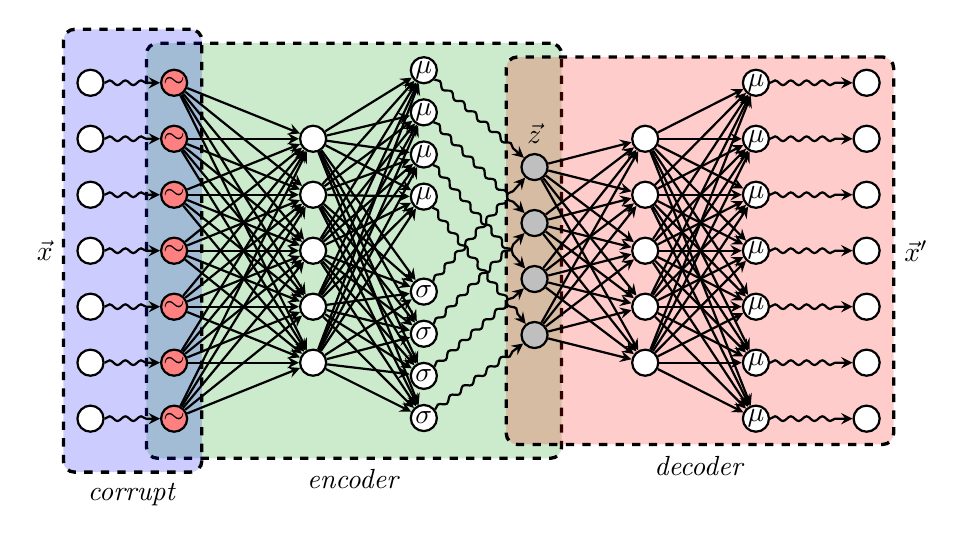
\begin{tikzpicture}

	\node (1) [draw, dashed, minimum height=15em, minimum width=15em, xshift=6.5em, fill=olivegreen, fill opacity=0.2, very thick, rectangle, rounded corners] {};
	\node (la1) [below=0em of 1] {\emph{encoder}};
	\node (2) [draw, dashed, minimum height=14em, fill = red, fill opacity=0.2,minimum width=14em, xshift=19em, very thick, rectangle, rounded corners] {};
	\node (la1) [below=0em of 2] {\emph{decoder}};
	\node (3) [draw, dashed, minimum height=16em, fill = blue, fill opacity=0.2,minimum width=5em, xshift=-1.5em, very thick, rectangle, rounded corners] {};
		\node (la3) [below=0em of 3] {\emph{corrupt}};
	
	\node[circle, thick, fill=red!50, draw] (x1) {};
	\node[circle, thick, draw, fill=red!50, below=1em of x1] (x2) {};
	\node[circle, thick, fill=red!50, draw, below=1em of x2] (x3) {};
	\node[circle, thick, fill=red!50, draw, below=1em of x3] (x4) {};
	\node[circle, thick, fill=red!50, draw, above=1em of x1] (x5) {};
	\node[circle, thick, fill=red!50, draw, above=1em of x5] (x6) {};
	\node[circle, thick, fill=red!50, draw, above=1em of x6] (x7) {};
	
	\foreach \x in {1,...,7}
		\node at (x\x) (lx\x) {$\sim$};
		
	\node[circle, thick, fill=white, left=2em of x1, draw] (i1) {};
	\node[circle, thick, draw, fill=white, below=1em of i1] (i2) {};
	\node[circle, thick, fill=white, draw, below=1em of i2] (i3) {};
	\node[circle, thick, fill=white, draw, below=1em of i3] (i4) {};
	\node[circle, thick, fill=white, draw, above=1em of i1] (i5) {};
	\node[circle, thick, fill=white, draw, above=1em of i5] (i6) {};
	\node[circle, thick, fill=white, draw, above=1em of i6] (i7) {};
	
	\foreach \x in {1,...,7}
		\draw[-stealth, decoration={snake, pre length=0.01mm, segment length=2mm, amplitude=0.3mm, post length=1.5mm}, decorate, thick] (i\x) -- (x\x);
	
	\node[circle, thick, right=4em of x1, fill=white, draw] (xh1) {};
	\node[circle, thick, draw, fill=white, below=1em of xh1] (xh2) {};
	\node[circle, thick, fill=white, draw, below=1em of xh2] (xh3) {};
	\node[circle, thick, fill=white, draw, above=1em of xh1] (xh4) {};
	\node[circle, thick, fill=white, draw, above=1em of xh4] (xh5) {};
	\node[circle, thick, fill=white, draw, right=8em of x1, yshift=5em] (hm1) {};
	\node[circle, thick, draw, fill=white, below=0.5em of hm1] (hm2) {};
	\node[circle, thick, draw, fill=white, below=0.5em of hm2] (hm3) {};
	\node[circle, thick, draw, fill=white, above=0.5em of hm1] (hm4) {};
	\node[circle, thick, fill=white, draw, right=8em of x1, yshift=-3em] (hs1) {};
	\node[circle, thick, draw, fill=white, below=0.5em of hs1] (hs2) {};
	\node[circle, thick, draw, fill=white, below=0.5em of hs2] (hs3) {};
	\node[circle, thick, draw, fill=white, above=0.5em of hs1] (hs4) {};
	\node[] at (hm1) (mu1) {$\mu$};
	\node[] at (hm2) (mu2) {$\mu$};
	\node[] at (hm3) (mu3) {$\mu$};
	\node[] at (hm4) (mu4) {$\mu$};
	\node[] at (hs1) (s1) {$\sigma$};
	\node[] at (hs2) (s2) {$\sigma$};
	\node[] at (hs3) (s3) {$\sigma$};
	\node[] at (hs4) (s4) {$\sigma$};
		
	\node[circle, thick, fill=lightgray, draw, right=12em of x1, yshift=1em] (h1) {};
	\node[circle, thick, draw, fill=lightgray, below=1em of h1] (h2) {};
	\node[circle, thick, draw, fill=lightgray, below=1em of h2] (h3) {};
	\node[circle, thick, draw, fill=lightgray, above=1em of h1] (h4) {};
	\node[circle, thick, right=16em of x1, fill=white, draw] (oh1) {};
	\node[circle, thick, draw, fill=white, below=1em of oh1] (oh2) {};
	\node[circle, thick, fill=white, draw, below=1em of oh2] (oh3) {};
	\node[circle, thick, fill=white, draw, above=1em of oh1] (oh4) {};
	\node[circle, thick, fill=white, draw, above=1em of oh4] (oh5) {};
	\node[circle, thick, draw, fill=white, right=20em of x1] (o1) {};
	\node[circle, thick, draw, fill=white, below=1em of o1] (o2) {};
	\node[circle, thick, draw, fill=white, below=1em of o2] (o3) {};
	\node[circle, thick, draw, fill=white, below=1em of o3] (o4) {};
	\node[circle, thick, draw, fill=white, above=1em of o1] (o5) {};
	\node[circle, thick, draw, fill=white, above=1em of o5] (o6) {};
	\node[circle, thick, draw, fill=white, above=1em of o6] (o7) {};
	\node[circle, thick, draw, fill=white, right=24em of x1] (oo1) {};
	\node[circle, thick, draw, fill=white, below=1em of oo1] (oo2) {};
	\node[circle, thick, draw, fill=white, below=1em of oo2] (oo3) {};
	\node[circle, thick, draw, fill=white, below=1em of oo3] (oo4) {};
	\node[circle, thick, draw, fill=white, above=1em of oo1] (oo5) {};
	\node[circle, thick, draw, fill=white, above=1em of oo5] (oo6) {};
	\node[circle, thick, draw, fill=white, above=1em of oo6] (oo7) {};
	\node[] at (o1) (muu1) {$\mu$};
	\node[] at (o2) (muu2) {$\mu$};
	\node[] at (o3) (muu3) {$\mu$};
	\node[] at (o4) (muu4) {$\mu$};
	\node[] at (o5) (muu5) {$\mu$};
	\node[] at (o6) (muu6) {$\mu$};
	\node[] at (o7) (muu7) {$\mu$};
	
	\foreach \x in {1,...,7}
		\foreach \y in {1,...,5}
			\draw[-stealth, thick] (x\x) -- (xh\y);
	
	\foreach \x in {1,...,5}
		\foreach \y in {1,...,4}
			\draw[-stealth, thick] (xh\x) -- (hm\y);
	
	\foreach \x in {1,...,5}
		\foreach \y in {1,...,4}
			\draw[-stealth, thick] (xh\x) -- (hs\y);
	
	\foreach \x in {1,...,4}
		\draw[-stealth, decoration={snake, pre length=0.01mm, segment length=2mm, amplitude=0.3mm, post length=1.5mm}, decorate, thick] (hs\x) -- (h\x);
	\foreach \x in {1,...,4}
		\draw[-stealth, decoration={snake, pre length=0.01mm, segment length=2mm, amplitude=0.3mm, post length=1.5mm}, decorate, thick] (hm\x) -- (h\x);
	
	\foreach \x in {1,...,5}
		\foreach \y in {1,...,4}
			\draw[-stealth, thick] (h\y) -- (oh\x);
	
	\foreach \x in {1,...,5}
		\foreach \y in {1,...,7}
			\draw[-stealth, thick] (oh\x) -- (o\y);
				
	\foreach \x in {1,...,7}
		\draw[-stealth, decoration={snake, pre length=0.01mm, segment length=2mm, amplitude=0.3mm, post length=1.5mm}, decorate, thick] (o\x) -- (oo\x);
				
	\node[left=0.5em of i1] (l1) {$\vec{x}$};
	\node[above=0em of h4] (l2) {$\vec{z}$};
	\node[right=0.5em of oo1] (l3) {$\vec{x}'$};

\end{tikzpicture}
\end{document}